\section{Experimental setup}
\label{sec:setup}
The sample of MB p--Pb collisions at $\snn$~=~5.02~TeV used for the present analysis was recorded using the ALICE detector in 2016. Due to the different energies of the proton and lead beams, the center-of-mass reference system in p--Pb collisions is shifted in rapidity by $\Delta y_{\mathrm{cms}} =$~0.465 along the direction of the proton beam. In the following, the convention that $y$ stands for $y_{\mathrm{cms}}$ is used. The ALICE apparatus used during the LHC Run 2 is described in detail in Ref.~\cite{Abelev:2014ffa}. The present analysis is carried out using the following detectors: the V0~\cite{ALICE:2013axi}, the Zero Degree Calorimeters (ZDC)~\cite{Cortese:2019nnv}, the Inner Tracking System (ITS)~\cite{ALICE:2010tia}, the Time Projection Chamber (TPC)~\cite{Alme:2010ke}, and the Time-Of-Flight (TOF)~\cite{Jacazio:2018slq}. 

The V0 detector consists of two arrays of scintillators located on both sides relative to the interaction point (IP), denoted as V0A and V0C, each made of 32 plastic scintillator strips, covering the full azimuthal angle within the pseudorapidity intervals $2.8 < \eta < 5.1$ and $-3.7 < \eta < -1.7$, respectively. Minimum bias p-Pb collisions are selected online by requiring a signal in both V0A and V0C detectors in coincidence with the arrival of the LHC bunch crossing. The total charge deposited in the V0A on the Pb-going side is utilized to define the multiplicity class. The collected MB sample corresponds to an integrated luminosity of 0.3~nb$^{-1}$~\cite{ALICE:2014gvw}. The ZDC detects nucleons emitted from the colliding nucleus by nuclear de-excitation processes or knocked out from wounded nucleons, the so-called “slow” nucleons. Two identical sets of the ZDC, each composed of a neutron (ZN) and a proton (ZP) calorimeters, are located at 112.5 m from the ALICE IP on both sides, covering very forward rapidity regions. The ZDC provides the least biased centrality selection in p--Pb collisions~\cite{ALICE:2014xsp}.

The primary vertex position is reconstructed using the measured track segments in the Silicon Pixel Detector (SPD)~\cite{Santoro2009:ALICESPD}, the innermost two layers of the ITS. The primary vertex along the beam direction ($z_\mathrm{vtx}$) is required to be in $|z_\mathrm{vtx}|<10$~cm from the nominal interaction point ($z_\mathrm{vtx}=0$). The pileup can be reduced by requiring the distance between the primary vertex and any additional reconstructed vertex to be larger than 0.8~cm. In addition, an inconsistency between the number of track candidates in the ITS and clusters in the SPD vetoes the pileup events~\cite{ALICE:2015olq}. After these selections, the probability of pileup events is expected to be about 0.1\% in the MB sample~\cite{ALICE:2017svf}. The TPC is the main tracking detector of ALICE, which covers the pseudorapidity range $|\eta|<$~0.9 over the full azimuth in a uniform solenoidal magnetic field of 0.5~T along the beam axis. The TPC is able to reconstruct charged particles down to $p_{\rm{T}}=$~0.15~GeV/$c$. Particle identification (PID) can be performed with the TPC and TOF. The TPC measures specific ionization energy loss $\mathrm{d}E/\mathrm{d}x$ of charged tracks to separate particle species. The TOF helps PID by measuring the flight time of charged particles from the primary vertex to the TOF.

\section{Data analysis}

The \fzero~resonances are reconstructed via the decay channel \fzero~$\rightarrow \pi^{+}\pi^{-}$, for which the branching ratio is reported to be B.R. = ($46\pm6$)\%~\cite{Stone:2013eaa}. \fzero~candidates are built from pairs of charged tracks reconstructed in the ITS and TPC. The tracks and required to have $p_{\mathrm{T}}>$~0.15~GeV/$c$ and $|\eta|<$~0.8 for a uniform detector acceptance. The reconstructed tracks are required to satisfy the standard selection criteria, as reported in~\cite{ALICE:2022qnb}, to guarantee that only tacks with high quality are selected. To ensure good track momentum resolution, the reconstructed tracks are required to have at least 70 readout pad crossed rows (out of a maximum of 159) in the TPC and two hits in the ITS (out of a maximum of 6), with at least one in the SPD. Selection criteria, which are dependent on $p_{\mathrm{T}}$, are applied to the distance of closest approach of the track to the primary vertex in the transverse ($d_{xy}$) and longitudinal ($d_{z}$) directions, requiring $|d_{z}|<$~2~cm and $|d_{xy}|<$~(0.0105~$+$~0.0350~$\times p_{\mathrm{T}}^{-1.1})$~cm ($p_{\mathrm{T}}$ in GeV/$c$), respectively, to suppress contamination from secondary charged particles originating from weakly decaying hadrons and interactions with the material.

The identification of charged pions is performed using the combined information of the TPC and TOF. The difference between the measured ionization energy loss and the expected value from a Bethe--Bloch parameterization obtained by assuming the particle is a pion is required to be within two standard deviations for the pion identification in the TPC. The difference between the measured flight time of the particle and the expected flight time for a pion is required to be within three standard deviations for the particle to be identified as a pion in the TOF. Tracks not having a signal associated in the TOF are identified using only the $\mathrm{d}E/\mathrm{d}x$ information from the TPC.

\label{sec:ana}
\begin{figure}[hbt!]
	\centering
	\subfigure{ 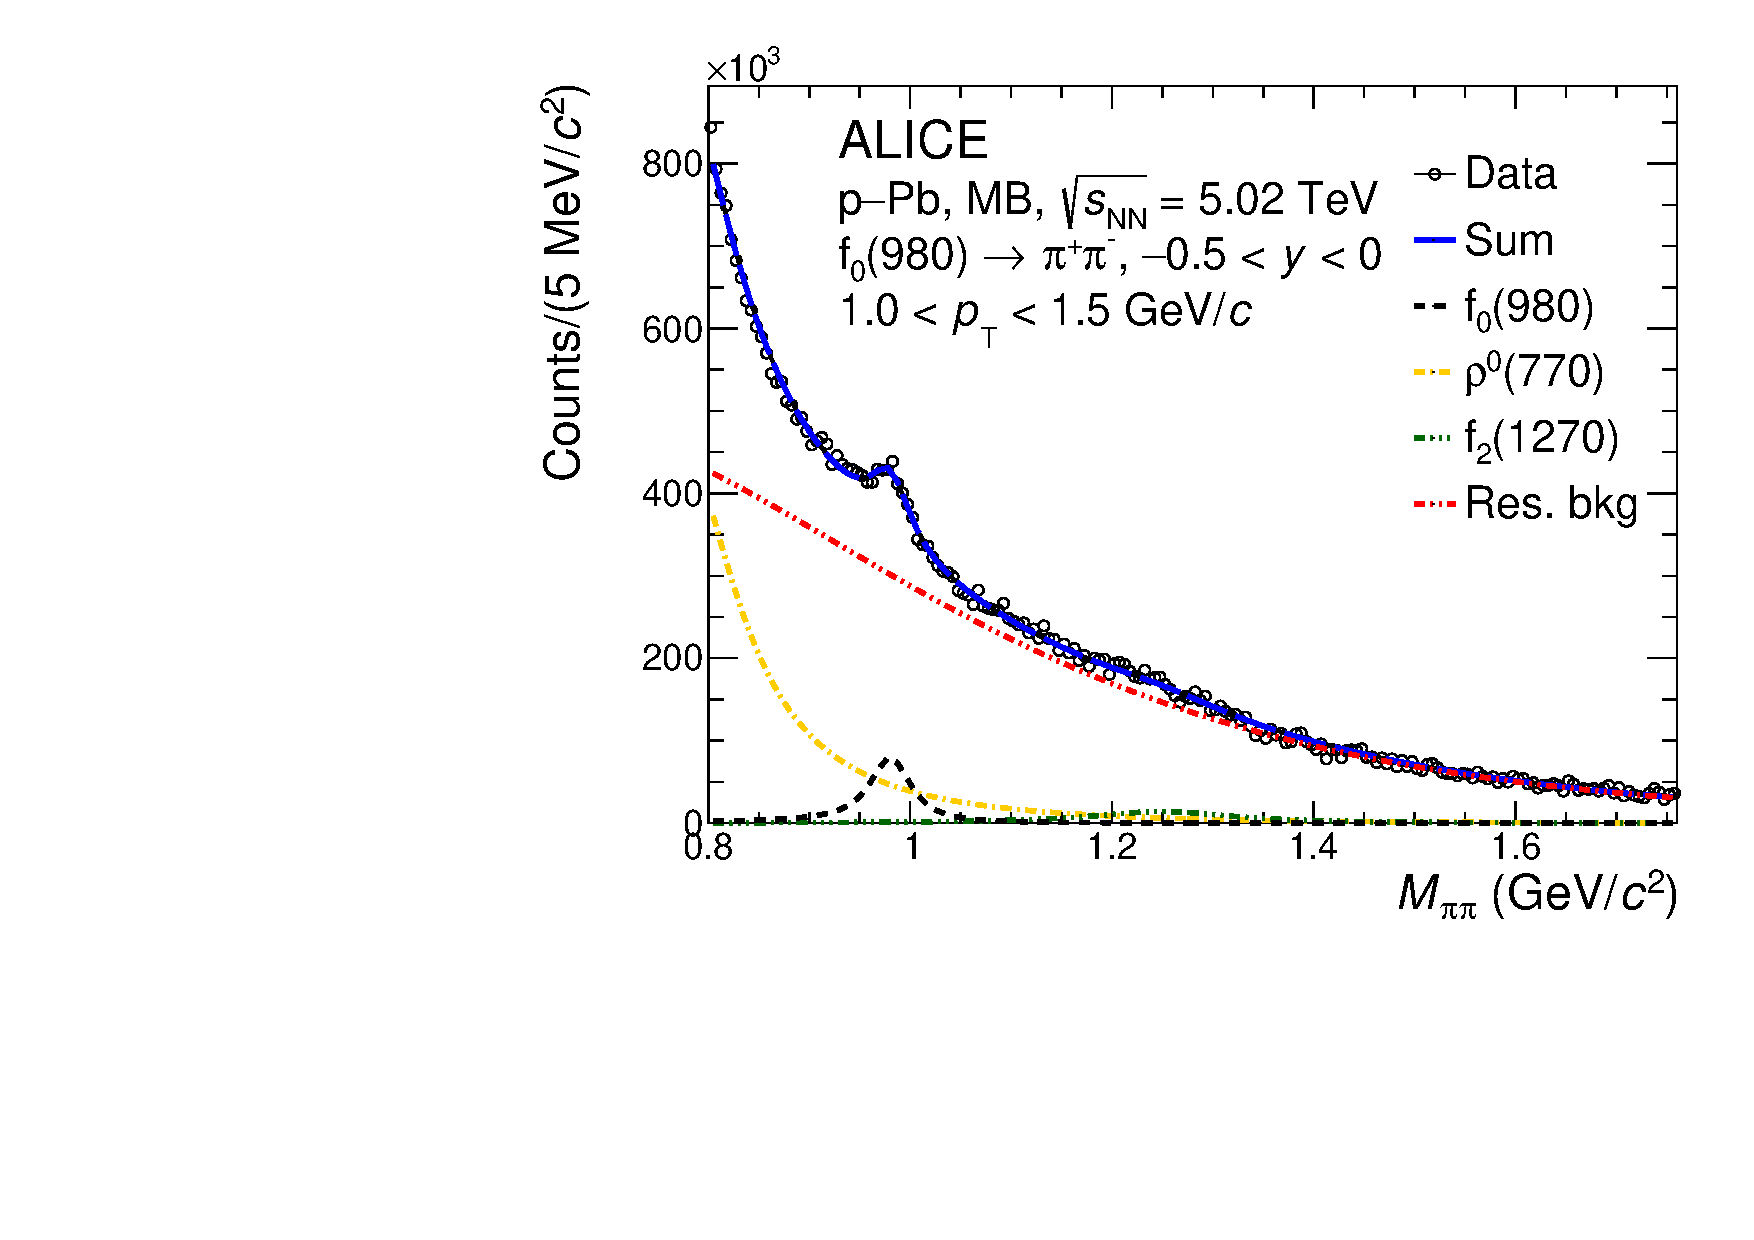
\includegraphics[width=0.47 \textwidth]{figures/Fig1_sigext_mb_pt0.pdf} }
	\subfigure{ 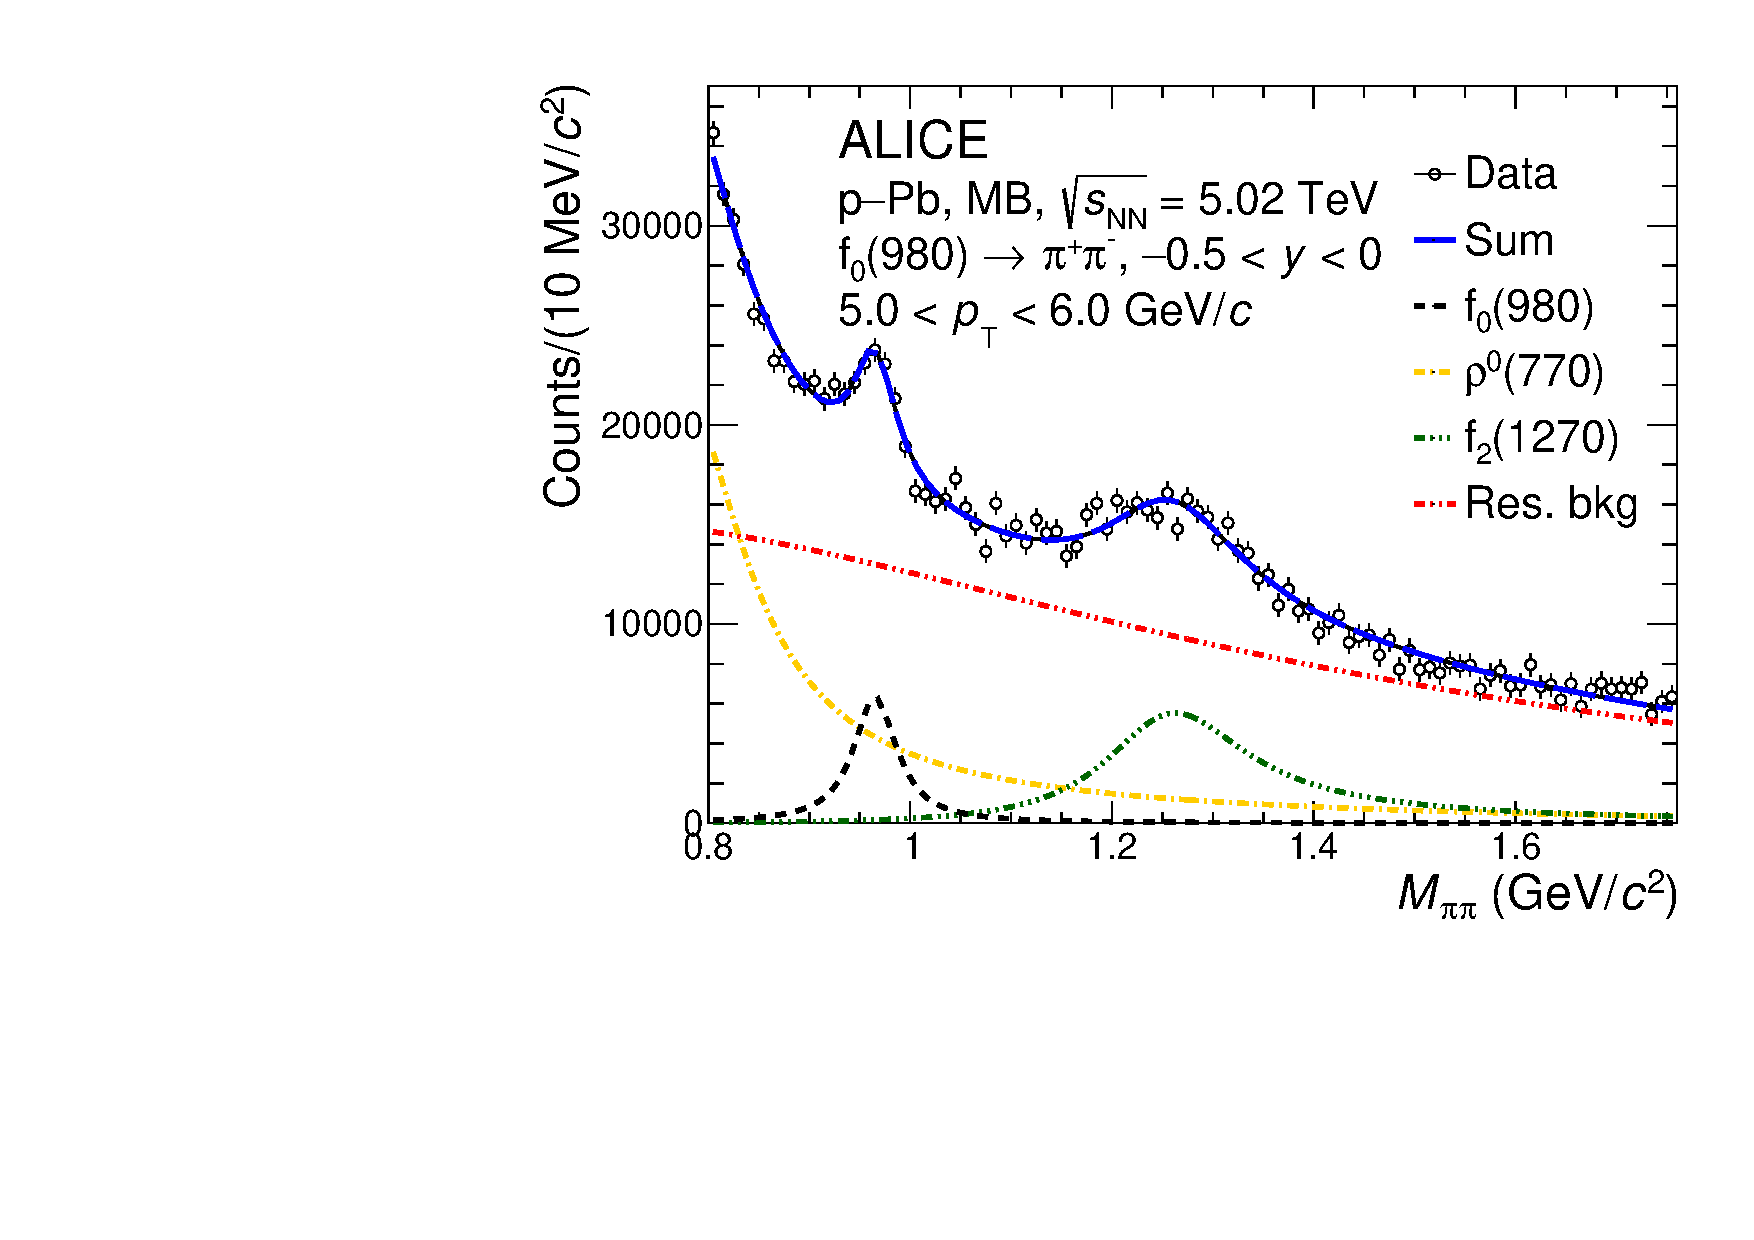
\includegraphics[width=0.47 \textwidth]{figures/Fig1_sigext_mb_pt1.pdf} }
	\caption{ Invariant mass distribution of $\pi^{+}\pi^{-}$ pairs in $-0.5<y<0$ after the like-sign background subtraction in p--Pb collisions at \snn~=~5.02~TeV. The left (right) plot is obtained at low (high) $p_{\mathrm{T}}$ of $\pi^{+}\pi^{-}$ pairs in minimum bias events. }
	\label{fig:SigExt}
\end{figure}

The \fzero~signals are extracted using an invariant mass analysis by associating two opposite-charge pions in the same event within $-0.5<y<0$~\cite{ALICE:2013wgn}. The combinatorial background is subtracted using the like-sign method~\cite{LIKESIGN}. The like-sign background is constructed as the geometric average of $\pi^{+}\pi^{+}$ and $\pi^{-}\pi^{-}$ distributions, 2$\sqrt{N_{\pi^{+}\pi^{+}}N_{\pi^{-}\pi^{-}}}$. After subtracting the like-sign background from the $\pi^{+}\pi^{-}$ distribution, peaks of resonances decaying to $\pi^{+}\pi^{-}$ can be identified. Figure~\ref{fig:SigExt} shows the like-sign-subtracted $\pi^{+}\pi^{-}$ invariant mass distributions for 1.0~$<p_{\rm{T}}<$~1.5~GeV/$c$ (5.0~$<p_{\rm{T}}<$~6.0~GeV/$c$) in MB events on the left (right) panel. Because \rhoz~and $\rm{f}_{2}$(1270) dominantly decay to $\pi^{+}\pi^{-}$ and have large widths, \fzero~signals are overlapped with contributions from those two resonances. In addition, a residual background ($f_{\mathrm{bkg}}$) is present, which is mainly attributed to misidentified particles and mini-jets. The measured invariant mass distribution is fitted with a function accounting for the contributions of this residual background and of the three resonances. Each resonance contribution is described with a relativistic Breit-Wigner function (rBW)~\cite{ALICE:2018qdv, ALICE:2022qnb}. Note that detector resolution gives a negligible contribution to the widths of broad resonances~\cite{ALICE:2016sak}. The rBW can be expressed as
\begin{eqnarray}
\mathrm{rBW}(M_{\pi\pi}) = \dfrac{AM_{\pi\pi}\Gamma(M_{\pi\pi})M_{0}}{(M_{\pi\pi}^{2}-M_{0}^{2})^{2} + M_{0}^{2}\Gamma^{2}(M_{\pi\pi})},
\label{eq:rBW}
\end{eqnarray}
where $\Gamma(M_{\pi\pi})$ is defined as
\begin{eqnarray}
\Gamma(M_{\pi\pi}) = \left[ \dfrac{ (M_{\pi\pi}^{2} - 4m_{\pi}^{2}) }{ (M_{0}^{2}-4m_{\pi}^{2}) } \right]^{(2J+1)/2} \times \dfrac{\Gamma_{0}M_{0}}{M_{\pi\pi}} .
\label{eq:rBWW}
\end{eqnarray}
Here, $A$ and $M_{0}$ are the amplitude of the rBW and the rest mass of the resonance, respectively. The rest width of the resonance, the spin, and the charged pion mass of 139.5~MeV/$c^{2}$ are represented as $\Gamma_{0}$, $J$, and $m_{\pi}$, respectively. The spins for \fzero, \rhoz, and $\mathrm{f}_{2}$(1270) are 0, 1, and 2, respectively. Each resonance rBW is corrected for the phase space~\cite{ALICE:2018qdv}, which can be expressed as
\begin{eqnarray}
\mathrm{PS}(M_{\pi\pi}) = \dfrac{M_{\pi\pi}}{\sqrt{M_{\pi\pi}^{2}+p_{\mathrm{T}}^{2}}}\times\exp{(-\sqrt{M_{\pi\pi}^{2}+p_{\mathrm{T}}^{2}}/T_{\mathrm{kin}})},
\label{eq:ps}
\end{eqnarray} 
where $p_{\mathrm{T}}$ in the above equation denotes the transverse momentum of the $\pi\pi$ pair and is set to be the median of each $p_{\mathrm{T}}$ interval, and $T_{\mathrm{kin}}$ is the kinetic freeze-out temperature, set to be 160~MeV~\cite{ALICE:2018qdv} for all the defined multiplicity classes. The $f_{\mathrm{bkg}}$ is modeled with a Maxwell-Boltzmann-like distribution, which can be expressed as~\cite{OPAL:1998enc}
\begin{eqnarray}
f_{\mathrm{bkg}}(M_{\pi\pi}) = B(M_{\pi\pi}-2m_{\pi})^{n}\exp{(c_{1}M_{\pi\pi} + c_{2}M_{\pi\pi}^{2})},
\label{eq:bkg}
\end{eqnarray} 
where, $B$, $n$, $c_{1}$, and $c_{2}$ are free parameters. 

The total fit function consists of the sum of three rBWs, one for each resonance and one function for the background, $f_{\mathrm{bkg}}$. This function has nine free parameters: three for \fzero~resonance (mass, width, and amplitude), two amplitudes for \rhoz~and f$_{2}$(1270) resonances, and four for $f_{\mathrm{bkg}}$. In particular, the width of the \fzero~which is not yet constrained by measurements (10~$<\Gamma_{0}^{\mathrm{f}_{0}}<$~100~MeV/$c^{2}$~\cite{ParticleDataGroup:2022pth}) is left as a free parameter in the fit. The masses and widths of \rhoz~and $\mathrm{f}_{2}$(1270) are fixed to their world-average values from Ref.~\cite{ParticleDataGroup:2022pth}, namely $m_{\rho}=$~775.3~MeV/$c^{2}$, $\Gamma^{\rho}_{0}=$~~149.1~MeV/$c^{2}$, $m_{\mathrm{f}_{2}}=$~1,275.5~MeV/$c^{2}$, and $\Gamma^{\mathrm{f}_{2}}_{0}=$~186.7~MeV/$c^{2}$. Due to the many free parameters in the fit function, the procedure is split into three steps to prevent parameter values from converging to local minima. The purpose of the first step is to obtain an unbiased and initial \fzero~width. This step is performed using the MB sample over a coarse $p_{\mathrm{T}}$ binning to reduce the effect of statistical fluctuations. The wider $p_{\mathrm{T}}$ binning is defined by merging 2-3 $p_{\mathrm{T}}$ bins of the original $p_{\mathrm{T}}$ binning. All nine parameters are left free in the first step. The second step aims at constraining the $f_{\mathrm{bkg}}$. The \fzero~width is fixed to the value determined from the wider $p_{\mathrm{T}}$ interval in the previous step for different multiplicity classes. The last fit procedure is processed fixing the parameters of $f_{\mathrm{bkg}}$ to those extracted in the previous step, while the \fzero~width is allowed to vary in the range of 10~$<\Gamma_{0}^{\mathrm{f}_{0}}<$~100~MeV/$c^{2}$. In this procedure, the amplitudes of the three resonances and the mass of the \fzero~are left free, and the fit range is set to 0.8~$<M_{\pi\pi}<$~1.76~GeV/$c^{2}$. In the last step, the extracted widths of \fzero~are about 40--70 MeV/$c^{2}$.


While for the \fzero~analysis performed in pp collisions~\cite{ALICE:2022qnb}, the width was constrained to be 55 MeV/$c^{2}$, the present analysis leaves the \fzero~width as a free parameter. In the previous analysis, no phase space correction was applied. On the other hand, the present analysis considers the phase space correction for a possibly larger probability of $\pi\pi$ interference~\cite{STAR:2003vqj} owing to higher multiplicity in p--Pb collisions. It is found that consistent invariant yields in pp collisions are obtained from the two different analysis methods.

Raw yields of \fzero~($N_{\mathrm{f}_{0}}$) are obtained by integrating the \fzero~rBW function in the measured $p_{\mathrm{T}}$ range and corrected for the acceptance, the tracking efficiency, and the PID efficiency and then normalized for the number of selected p--Pb collisions and the B.R.~\cite{Stone:2013eaa}. The fully corrected yield can be expressed as
\begin{eqnarray}
\dfrac{1}{N_{\mathrm{NSD}}}\dfrac{\mathrm{d}^{2}N}{\mathrm{dyd}p_{\mathrm{T}}} = \dfrac{1}{N_{\mathrm{evt}}} \dfrac{ N_{\mathrm{f}_{0}} }{ \Delta y \Delta p_{\mathrm{T}} } \dfrac{  \epsilon_{\mathrm{trig}} f_{\mathrm{vtx}} f_{\mathrm{SL}} }{\mathrm{Acc} \times \epsilon \times \mathrm{B.R.} }.
\end{eqnarray}
Here, the number of events satisfying the event selection criteria in the specific multiplicity class is represented as $N_{\mathrm{evt}}$ and is normalized to $N_{\mathrm{NSD}}$, which is the number of non-single diffractive (NSD) events. The width of the rapidity interval (of 0.5 units) is represented as $\Delta y$. Coefficients for the acceptance ($\mathrm{Acc}$) and the efficiency ($\epsilon$) of the tracking and PID for pion pairs are estimated from a detailed simulation of the ALICE detector response. The p--Pb collisions are simulated using the DPMJET~\cite{Fedynitch:2015kcn} event generator with the injection of \fzero~signals. The generated particles (signal and background) are transported through the detector using GEANT3~\cite{Brun:1994aa}. The $\mathrm{Acc}\times\epsilon$ is estimated to be 26\% in the 0~$<p_{\mathrm{T}}<$~0.3~GeV/$c$ interval and gradually increasing up to 60\% as $p_{\mathrm{T}}$ increases and it is not dependent on the multiplicity class. The $\mathrm{B.R.}$ is the branching ratio of the \fzero~$\rightarrow \pi^{+}\pi^{-}$ decay channel. The \fzero~yield is normalized for the trigger efficiency ($\epsilon_{\mathrm{trig}}$), vertex reconstruction efficiency ($f_{\mathrm{vtx}}$), and signal loss ($f_{\mathrm{SL}}$) due to the event selection. The $\epsilon_{\mathrm{trig}}$ depends on the multiplicity class increasing from 0.84 to 1 as the multiplicity increases. The $f_{\mathrm{vtx}}$ is estimated to be larger than 0.99 in all measured multiplicity classes. The $f_{\mathrm{SL}}$ corrects for the \fzero~signal loss due to the event selection. Because general Monte Carlo event generators do not generate primary \fzero, the $f_{\mathrm{SL}}$ is estimated using a different particle, the $\phi$ meson, exploiting the universal $m_{\mathrm{T}}$ scaling~\cite{Altenkamper:2017qot}. This approach shows that $f_{\mathrm{SL}}$ does not depend on particle species~\cite{ALICE:2019xyr}, and it is found to be 1.03 for 0~$<p_{\mathrm{T}}<$~0.3~GeV/$c$ and approaching unity for $p_{\mathrm{T}}>$~2~GeV/$c$.

\section{Systematic uncertainties}
\label{sec:syst}
The systematic uncertainties of the \fzero~yields are estimated by varying the analysis selection criteria, the configuration of the fit used to extract the raw yield, and the treatment of the phase space correction. The estimated uncertainties are summarized in Tab.~\ref{tab:syst}. The total systematic uncertainty is calculated as the quadratic sum of the different contributing sources. Each uncertainty is aimlessly varying with the multiplicity class and the $p_{\mathrm{T}}$ range and is represented as the minimum and maximum values of the observed variation. The relative uncertainty of the $\mathrm{B.R.}$ on the invariant yields is 13\%~\cite{Stone:2013eaa} and is not included in the total uncertainty.

\begin{table}[h!]
\caption{Relative systematic uncertainties of the \fzero~$p_{\rm{T}}$-differential yields. Numbers given in ranges correspond to minimum and maximum uncertainties.}
\centering
\begin{tabular}{l|c}
\hline 
Sources &Systematic uncertainty (\%) \\ \hline
Primary vertex &negligible \\ 
Pileup rejection & negligible \\ 
Tracking & 4 \\
Particle identification & 4--12 \\ 
$\mathrm{f}_{2}$(1270) parameters	& 3--9 \\ 
\rhoz~parameters & 3--8 \\
Fit range & 0--6 \\
Initial $\mathrm{f}_{0}$ width & 2--12 \\
Phase space correction & 3--8 \\ \hline 
Total (in quadrature)	& 15--27 \\ 
\hline 
\end{tabular}
\label{tab:syst}
\end{table}

The systematic uncertainty from the primary vertex selection is estimated by repeating the analysis with a different selection of $|z_\mathrm{vtx}|<$~7~cm and found to be negligible. The systematic uncertainty from the pileup rejection is tested by varying the minimum number of track segments contributing to the reconstruction of pileup collision vertices from 5 to 3. The uncertainty is estimated to be negligible.

The systematic uncertainty from tracking is taken from~\cite{ALICE:2013wgn}, where uncertainties are evaluated by varying the requirements to select reconstructed tracks such as $d_{xy}$, $d_{z}$, and the number of crossed rows. The estimated uncertainty is 4\%. The systematic uncertainty from the PID is tested with different requirements on the number of standard deviations ($\pm\,0.5\sigma$ with respect to the default selections) for the TPC and TOF. The uncertainties are estimated to be 4--12\%.

The uncertainties due to the \fzero~yield extraction via the fits to the invariant mass distributions are estimated by varying some of the configurations in the fit procedure. The contributions coming from masses and widths of $\mathrm{f}_{2}$(1270) and \rhoz~are evaluated by shifting the masses and the widths by three standard deviations with respect to their world-average values using the uncertainties reported at Ref.~\cite{ParticleDataGroup:2022pth}. The estimated systematic uncertainties are 3--9\% and 3--8\%, respectively. Furthermore, the invariant mass range used in the fit is changed inward or outward by 40~MeV$/c^{2}$, and the resulting systematic uncertainty is found to be less than 6\%. The contribution from the initial guess for the \fzero~width value, which is obtained in the first step described in Sec.~\ref{sec:ana}, is estimated by varying the width within the statistical uncertainties, which is about 5~MeV/$c{^2}$ in average, in both directions. The variations affect the background distribution determined in the second step, and the estimated systematic uncertainties are 2--12\%. The systematic uncertainty from the phase space correction is estimated by varying the kinetic freeze-out temperature in the range of 140~$<T_{\mathrm{kin}}<$~180~MeV. The estimated uncertainties are 3--8\%. 

The correlations of systematic uncertainties along the multiplicity class are quantified. The uncertainty is considered more closely correlated when the directions of systematic deviations are same for different multiplicity classes. The directions of systematic deviations are compared between a given multiplicity class and the MB class. The test is applied to all systematic uncertainties and concludes that approximately half of the total systematic uncertainties are uncorrelated.